    
\documentclass[11pt]{article}

    
    \usepackage[breakable]{tcolorbox}
    \tcbset{nobeforeafter} % prevents tcolorboxes being placing in paragraphs
    \usepackage{float}
    \floatplacement{figure}{H} % forces figures to be placed at the correct location
    
    \usepackage[T1]{fontenc}
    % Nicer default font (+ math font) than Computer Modern for most use cases
    \usepackage{mathpazo}

    % Basic figure setup, for now with no caption control since it's done
    % automatically by Pandoc (which extracts ![](path) syntax from Markdown).
    \usepackage{graphicx}
    % We will generate all images so they have a width \maxwidth. This means
    % that they will get their normal width if they fit onto the page, but
    % are scaled down if they would overflow the margins.
    \makeatletter
    \def\maxwidth{\ifdim\Gin@nat@width>\linewidth\linewidth
    \else\Gin@nat@width\fi}
    \makeatother
    \let\Oldincludegraphics\includegraphics
    % Set max figure width to be 80% of text width, for now hardcoded.
    \renewcommand{\includegraphics}[1]{\Oldincludegraphics[width=.8\maxwidth]{#1}}
    % Ensure that by default, figures have no caption (until we provide a
    % proper Figure object with a Caption API and a way to capture that
    % in the conversion process - todo).
    \usepackage{caption}
    \DeclareCaptionLabelFormat{nolabel}{}
    \captionsetup{labelformat=nolabel}

    \usepackage{adjustbox} % Used to constrain images to a maximum size 
    \usepackage{xcolor} % Allow colors to be defined
    \usepackage{enumerate} % Needed for markdown enumerations to work
    \usepackage{geometry} % Used to adjust the document margins
    \usepackage{amsmath} % Equations
    \usepackage{amssymb} % Equations
    \usepackage{textcomp} % defines textquotesingle
    % Hack from http://tex.stackexchange.com/a/47451/13684:
    \AtBeginDocument{%
        \def\PYZsq{\textquotesingle}% Upright quotes in Pygmentized code
    }
    \usepackage{upquote} % Upright quotes for verbatim code
    \usepackage{eurosym} % defines \euro
    \usepackage[mathletters]{ucs} % Extended unicode (utf-8) support
    \usepackage[utf8x]{inputenc} % Allow utf-8 characters in the tex document
    \usepackage{fancyvrb} % verbatim replacement that allows latex
    \usepackage{grffile} % extends the file name processing of package graphics 
                         % to support a larger range 
    % The hyperref package gives us a pdf with properly built
    % internal navigation ('pdf bookmarks' for the table of contents,
    % internal cross-reference links, web links for URLs, etc.)
    \usepackage{hyperref}
    \usepackage{longtable} % longtable support required by pandoc >1.10
    \usepackage{booktabs}  % table support for pandoc > 1.12.2
    \usepackage[inline]{enumitem} % IRkernel/repr support (it uses the enumerate* environment)
    \usepackage[normalem]{ulem} % ulem is needed to support strikethroughs (\sout)
                                % normalem makes italics be italics, not underlines
    \usepackage{mathrsfs}
    

    
    % Colors for the hyperref package
    \definecolor{urlcolor}{rgb}{0,.145,.698}
    \definecolor{linkcolor}{rgb}{.71,0.21,0.01}
    \definecolor{citecolor}{rgb}{.12,.54,.11}

    % ANSI colors
    \definecolor{ansi-black}{HTML}{3E424D}
    \definecolor{ansi-black-intense}{HTML}{282C36}
    \definecolor{ansi-red}{HTML}{E75C58}
    \definecolor{ansi-red-intense}{HTML}{B22B31}
    \definecolor{ansi-green}{HTML}{00A250}
    \definecolor{ansi-green-intense}{HTML}{007427}
    \definecolor{ansi-yellow}{HTML}{DDB62B}
    \definecolor{ansi-yellow-intense}{HTML}{B27D12}
    \definecolor{ansi-blue}{HTML}{208FFB}
    \definecolor{ansi-blue-intense}{HTML}{0065CA}
    \definecolor{ansi-magenta}{HTML}{D160C4}
    \definecolor{ansi-magenta-intense}{HTML}{A03196}
    \definecolor{ansi-cyan}{HTML}{60C6C8}
    \definecolor{ansi-cyan-intense}{HTML}{258F8F}
    \definecolor{ansi-white}{HTML}{C5C1B4}
    \definecolor{ansi-white-intense}{HTML}{A1A6B2}
    \definecolor{ansi-default-inverse-fg}{HTML}{FFFFFF}
    \definecolor{ansi-default-inverse-bg}{HTML}{000000}

    % commands and environments needed by pandoc snippets
    % extracted from the output of `pandoc -s`
    \providecommand{\tightlist}{%
      \setlength{\itemsep}{0pt}\setlength{\parskip}{0pt}}
    \DefineVerbatimEnvironment{Highlighting}{Verbatim}{commandchars=\\\{\}}
    % Add ',fontsize=\small' for more characters per line
    \newenvironment{Shaded}{}{}
    \newcommand{\KeywordTok}[1]{\textcolor[rgb]{0.00,0.44,0.13}{\textbf{{#1}}}}
    \newcommand{\DataTypeTok}[1]{\textcolor[rgb]{0.56,0.13,0.00}{{#1}}}
    \newcommand{\DecValTok}[1]{\textcolor[rgb]{0.25,0.63,0.44}{{#1}}}
    \newcommand{\BaseNTok}[1]{\textcolor[rgb]{0.25,0.63,0.44}{{#1}}}
    \newcommand{\FloatTok}[1]{\textcolor[rgb]{0.25,0.63,0.44}{{#1}}}
    \newcommand{\CharTok}[1]{\textcolor[rgb]{0.25,0.44,0.63}{{#1}}}
    \newcommand{\StringTok}[1]{\textcolor[rgb]{0.25,0.44,0.63}{{#1}}}
    \newcommand{\CommentTok}[1]{\textcolor[rgb]{0.38,0.63,0.69}{\textit{{#1}}}}
    \newcommand{\OtherTok}[1]{\textcolor[rgb]{0.00,0.44,0.13}{{#1}}}
    \newcommand{\AlertTok}[1]{\textcolor[rgb]{1.00,0.00,0.00}{\textbf{{#1}}}}
    \newcommand{\FunctionTok}[1]{\textcolor[rgb]{0.02,0.16,0.49}{{#1}}}
    \newcommand{\RegionMarkerTok}[1]{{#1}}
    \newcommand{\ErrorTok}[1]{\textcolor[rgb]{1.00,0.00,0.00}{\textbf{{#1}}}}
    \newcommand{\NormalTok}[1]{{#1}}
    
    % Additional commands for more recent versions of Pandoc
    \newcommand{\ConstantTok}[1]{\textcolor[rgb]{0.53,0.00,0.00}{{#1}}}
    \newcommand{\SpecialCharTok}[1]{\textcolor[rgb]{0.25,0.44,0.63}{{#1}}}
    \newcommand{\VerbatimStringTok}[1]{\textcolor[rgb]{0.25,0.44,0.63}{{#1}}}
    \newcommand{\SpecialStringTok}[1]{\textcolor[rgb]{0.73,0.40,0.53}{{#1}}}
    \newcommand{\ImportTok}[1]{{#1}}
    \newcommand{\DocumentationTok}[1]{\textcolor[rgb]{0.73,0.13,0.13}{\textit{{#1}}}}
    \newcommand{\AnnotationTok}[1]{\textcolor[rgb]{0.38,0.63,0.69}{\textbf{\textit{{#1}}}}}
    \newcommand{\CommentVarTok}[1]{\textcolor[rgb]{0.38,0.63,0.69}{\textbf{\textit{{#1}}}}}
    \newcommand{\VariableTok}[1]{\textcolor[rgb]{0.10,0.09,0.49}{{#1}}}
    \newcommand{\ControlFlowTok}[1]{\textcolor[rgb]{0.00,0.44,0.13}{\textbf{{#1}}}}
    \newcommand{\OperatorTok}[1]{\textcolor[rgb]{0.40,0.40,0.40}{{#1}}}
    \newcommand{\BuiltInTok}[1]{{#1}}
    \newcommand{\ExtensionTok}[1]{{#1}}
    \newcommand{\PreprocessorTok}[1]{\textcolor[rgb]{0.74,0.48,0.00}{{#1}}}
    \newcommand{\AttributeTok}[1]{\textcolor[rgb]{0.49,0.56,0.16}{{#1}}}
    \newcommand{\InformationTok}[1]{\textcolor[rgb]{0.38,0.63,0.69}{\textbf{\textit{{#1}}}}}
    \newcommand{\WarningTok}[1]{\textcolor[rgb]{0.38,0.63,0.69}{\textbf{\textit{{#1}}}}}
    
    
    % Define a nice break command that doesn't care if a line doesn't already
    % exist.
    \def\br{\hspace*{\fill} \\* }
    % Math Jax compatibility definitions
    \def\gt{>}
    \def\lt{<}
    \let\Oldtex\TeX
    \let\Oldlatex\LaTeX
    \renewcommand{\TeX}{\textrm{\Oldtex}}
    \renewcommand{\LaTeX}{\textrm{\Oldlatex}}
    % Document parameters
    % Document title
    \title{III.4 Cadenas de Markov}

    
% Pygments definitions
\makeatletter
\def\PY@reset{\let\PY@it=\relax \let\PY@bf=\relax%
    \let\PY@ul=\relax \let\PY@tc=\relax%
    \let\PY@bc=\relax \let\PY@ff=\relax}
\def\PY@tok#1{\csname PY@tok@#1\endcsname}
\def\PY@toks#1+{\ifx\relax#1\empty\else%
    \PY@tok{#1}\expandafter\PY@toks\fi}
\def\PY@do#1{\PY@bc{\PY@tc{\PY@ul{%
    \PY@it{\PY@bf{\PY@ff{#1}}}}}}}
\def\PY#1#2{\PY@reset\PY@toks#1+\relax+\PY@do{#2}}

\expandafter\def\csname PY@tok@w\endcsname{\def\PY@tc##1{\textcolor[rgb]{0.73,0.73,0.73}{##1}}}
\expandafter\def\csname PY@tok@c\endcsname{\let\PY@it=\textit\def\PY@tc##1{\textcolor[rgb]{0.25,0.50,0.50}{##1}}}
\expandafter\def\csname PY@tok@cp\endcsname{\def\PY@tc##1{\textcolor[rgb]{0.74,0.48,0.00}{##1}}}
\expandafter\def\csname PY@tok@k\endcsname{\let\PY@bf=\textbf\def\PY@tc##1{\textcolor[rgb]{0.00,0.50,0.00}{##1}}}
\expandafter\def\csname PY@tok@kp\endcsname{\def\PY@tc##1{\textcolor[rgb]{0.00,0.50,0.00}{##1}}}
\expandafter\def\csname PY@tok@kt\endcsname{\def\PY@tc##1{\textcolor[rgb]{0.69,0.00,0.25}{##1}}}
\expandafter\def\csname PY@tok@o\endcsname{\def\PY@tc##1{\textcolor[rgb]{0.40,0.40,0.40}{##1}}}
\expandafter\def\csname PY@tok@ow\endcsname{\let\PY@bf=\textbf\def\PY@tc##1{\textcolor[rgb]{0.67,0.13,1.00}{##1}}}
\expandafter\def\csname PY@tok@nb\endcsname{\def\PY@tc##1{\textcolor[rgb]{0.00,0.50,0.00}{##1}}}
\expandafter\def\csname PY@tok@nf\endcsname{\def\PY@tc##1{\textcolor[rgb]{0.00,0.00,1.00}{##1}}}
\expandafter\def\csname PY@tok@nc\endcsname{\let\PY@bf=\textbf\def\PY@tc##1{\textcolor[rgb]{0.00,0.00,1.00}{##1}}}
\expandafter\def\csname PY@tok@nn\endcsname{\let\PY@bf=\textbf\def\PY@tc##1{\textcolor[rgb]{0.00,0.00,1.00}{##1}}}
\expandafter\def\csname PY@tok@ne\endcsname{\let\PY@bf=\textbf\def\PY@tc##1{\textcolor[rgb]{0.82,0.25,0.23}{##1}}}
\expandafter\def\csname PY@tok@nv\endcsname{\def\PY@tc##1{\textcolor[rgb]{0.10,0.09,0.49}{##1}}}
\expandafter\def\csname PY@tok@no\endcsname{\def\PY@tc##1{\textcolor[rgb]{0.53,0.00,0.00}{##1}}}
\expandafter\def\csname PY@tok@nl\endcsname{\def\PY@tc##1{\textcolor[rgb]{0.63,0.63,0.00}{##1}}}
\expandafter\def\csname PY@tok@ni\endcsname{\let\PY@bf=\textbf\def\PY@tc##1{\textcolor[rgb]{0.60,0.60,0.60}{##1}}}
\expandafter\def\csname PY@tok@na\endcsname{\def\PY@tc##1{\textcolor[rgb]{0.49,0.56,0.16}{##1}}}
\expandafter\def\csname PY@tok@nt\endcsname{\let\PY@bf=\textbf\def\PY@tc##1{\textcolor[rgb]{0.00,0.50,0.00}{##1}}}
\expandafter\def\csname PY@tok@nd\endcsname{\def\PY@tc##1{\textcolor[rgb]{0.67,0.13,1.00}{##1}}}
\expandafter\def\csname PY@tok@s\endcsname{\def\PY@tc##1{\textcolor[rgb]{0.73,0.13,0.13}{##1}}}
\expandafter\def\csname PY@tok@sd\endcsname{\let\PY@it=\textit\def\PY@tc##1{\textcolor[rgb]{0.73,0.13,0.13}{##1}}}
\expandafter\def\csname PY@tok@si\endcsname{\let\PY@bf=\textbf\def\PY@tc##1{\textcolor[rgb]{0.73,0.40,0.53}{##1}}}
\expandafter\def\csname PY@tok@se\endcsname{\let\PY@bf=\textbf\def\PY@tc##1{\textcolor[rgb]{0.73,0.40,0.13}{##1}}}
\expandafter\def\csname PY@tok@sr\endcsname{\def\PY@tc##1{\textcolor[rgb]{0.73,0.40,0.53}{##1}}}
\expandafter\def\csname PY@tok@ss\endcsname{\def\PY@tc##1{\textcolor[rgb]{0.10,0.09,0.49}{##1}}}
\expandafter\def\csname PY@tok@sx\endcsname{\def\PY@tc##1{\textcolor[rgb]{0.00,0.50,0.00}{##1}}}
\expandafter\def\csname PY@tok@m\endcsname{\def\PY@tc##1{\textcolor[rgb]{0.40,0.40,0.40}{##1}}}
\expandafter\def\csname PY@tok@gh\endcsname{\let\PY@bf=\textbf\def\PY@tc##1{\textcolor[rgb]{0.00,0.00,0.50}{##1}}}
\expandafter\def\csname PY@tok@gu\endcsname{\let\PY@bf=\textbf\def\PY@tc##1{\textcolor[rgb]{0.50,0.00,0.50}{##1}}}
\expandafter\def\csname PY@tok@gd\endcsname{\def\PY@tc##1{\textcolor[rgb]{0.63,0.00,0.00}{##1}}}
\expandafter\def\csname PY@tok@gi\endcsname{\def\PY@tc##1{\textcolor[rgb]{0.00,0.63,0.00}{##1}}}
\expandafter\def\csname PY@tok@gr\endcsname{\def\PY@tc##1{\textcolor[rgb]{1.00,0.00,0.00}{##1}}}
\expandafter\def\csname PY@tok@ge\endcsname{\let\PY@it=\textit}
\expandafter\def\csname PY@tok@gs\endcsname{\let\PY@bf=\textbf}
\expandafter\def\csname PY@tok@gp\endcsname{\let\PY@bf=\textbf\def\PY@tc##1{\textcolor[rgb]{0.00,0.00,0.50}{##1}}}
\expandafter\def\csname PY@tok@go\endcsname{\def\PY@tc##1{\textcolor[rgb]{0.53,0.53,0.53}{##1}}}
\expandafter\def\csname PY@tok@gt\endcsname{\def\PY@tc##1{\textcolor[rgb]{0.00,0.27,0.87}{##1}}}
\expandafter\def\csname PY@tok@err\endcsname{\def\PY@bc##1{\setlength{\fboxsep}{0pt}\fcolorbox[rgb]{1.00,0.00,0.00}{1,1,1}{\strut ##1}}}
\expandafter\def\csname PY@tok@kc\endcsname{\let\PY@bf=\textbf\def\PY@tc##1{\textcolor[rgb]{0.00,0.50,0.00}{##1}}}
\expandafter\def\csname PY@tok@kd\endcsname{\let\PY@bf=\textbf\def\PY@tc##1{\textcolor[rgb]{0.00,0.50,0.00}{##1}}}
\expandafter\def\csname PY@tok@kn\endcsname{\let\PY@bf=\textbf\def\PY@tc##1{\textcolor[rgb]{0.00,0.50,0.00}{##1}}}
\expandafter\def\csname PY@tok@kr\endcsname{\let\PY@bf=\textbf\def\PY@tc##1{\textcolor[rgb]{0.00,0.50,0.00}{##1}}}
\expandafter\def\csname PY@tok@bp\endcsname{\def\PY@tc##1{\textcolor[rgb]{0.00,0.50,0.00}{##1}}}
\expandafter\def\csname PY@tok@fm\endcsname{\def\PY@tc##1{\textcolor[rgb]{0.00,0.00,1.00}{##1}}}
\expandafter\def\csname PY@tok@vc\endcsname{\def\PY@tc##1{\textcolor[rgb]{0.10,0.09,0.49}{##1}}}
\expandafter\def\csname PY@tok@vg\endcsname{\def\PY@tc##1{\textcolor[rgb]{0.10,0.09,0.49}{##1}}}
\expandafter\def\csname PY@tok@vi\endcsname{\def\PY@tc##1{\textcolor[rgb]{0.10,0.09,0.49}{##1}}}
\expandafter\def\csname PY@tok@vm\endcsname{\def\PY@tc##1{\textcolor[rgb]{0.10,0.09,0.49}{##1}}}
\expandafter\def\csname PY@tok@sa\endcsname{\def\PY@tc##1{\textcolor[rgb]{0.73,0.13,0.13}{##1}}}
\expandafter\def\csname PY@tok@sb\endcsname{\def\PY@tc##1{\textcolor[rgb]{0.73,0.13,0.13}{##1}}}
\expandafter\def\csname PY@tok@sc\endcsname{\def\PY@tc##1{\textcolor[rgb]{0.73,0.13,0.13}{##1}}}
\expandafter\def\csname PY@tok@dl\endcsname{\def\PY@tc##1{\textcolor[rgb]{0.73,0.13,0.13}{##1}}}
\expandafter\def\csname PY@tok@s2\endcsname{\def\PY@tc##1{\textcolor[rgb]{0.73,0.13,0.13}{##1}}}
\expandafter\def\csname PY@tok@sh\endcsname{\def\PY@tc##1{\textcolor[rgb]{0.73,0.13,0.13}{##1}}}
\expandafter\def\csname PY@tok@s1\endcsname{\def\PY@tc##1{\textcolor[rgb]{0.73,0.13,0.13}{##1}}}
\expandafter\def\csname PY@tok@mb\endcsname{\def\PY@tc##1{\textcolor[rgb]{0.40,0.40,0.40}{##1}}}
\expandafter\def\csname PY@tok@mf\endcsname{\def\PY@tc##1{\textcolor[rgb]{0.40,0.40,0.40}{##1}}}
\expandafter\def\csname PY@tok@mh\endcsname{\def\PY@tc##1{\textcolor[rgb]{0.40,0.40,0.40}{##1}}}
\expandafter\def\csname PY@tok@mi\endcsname{\def\PY@tc##1{\textcolor[rgb]{0.40,0.40,0.40}{##1}}}
\expandafter\def\csname PY@tok@il\endcsname{\def\PY@tc##1{\textcolor[rgb]{0.40,0.40,0.40}{##1}}}
\expandafter\def\csname PY@tok@mo\endcsname{\def\PY@tc##1{\textcolor[rgb]{0.40,0.40,0.40}{##1}}}
\expandafter\def\csname PY@tok@ch\endcsname{\let\PY@it=\textit\def\PY@tc##1{\textcolor[rgb]{0.25,0.50,0.50}{##1}}}
\expandafter\def\csname PY@tok@cm\endcsname{\let\PY@it=\textit\def\PY@tc##1{\textcolor[rgb]{0.25,0.50,0.50}{##1}}}
\expandafter\def\csname PY@tok@cpf\endcsname{\let\PY@it=\textit\def\PY@tc##1{\textcolor[rgb]{0.25,0.50,0.50}{##1}}}
\expandafter\def\csname PY@tok@c1\endcsname{\let\PY@it=\textit\def\PY@tc##1{\textcolor[rgb]{0.25,0.50,0.50}{##1}}}
\expandafter\def\csname PY@tok@cs\endcsname{\let\PY@it=\textit\def\PY@tc##1{\textcolor[rgb]{0.25,0.50,0.50}{##1}}}

\def\PYZbs{\char`\\}
\def\PYZus{\char`\_}
\def\PYZob{\char`\{}
\def\PYZcb{\char`\}}
\def\PYZca{\char`\^}
\def\PYZam{\char`\&}
\def\PYZlt{\char`\<}
\def\PYZgt{\char`\>}
\def\PYZsh{\char`\#}
\def\PYZpc{\char`\%}
\def\PYZdl{\char`\$}
\def\PYZhy{\char`\-}
\def\PYZsq{\char`\'}
\def\PYZdq{\char`\"}
\def\PYZti{\char`\~}
% for compatibility with earlier versions
\def\PYZat{@}
\def\PYZlb{[}
\def\PYZrb{]}
\makeatother


    % For linebreaks inside Verbatim environment from package fancyvrb. 
    \makeatletter
        \newbox\Wrappedcontinuationbox 
        \newbox\Wrappedvisiblespacebox 
        \newcommand*\Wrappedvisiblespace {\textcolor{red}{\textvisiblespace}} 
        \newcommand*\Wrappedcontinuationsymbol {\textcolor{red}{\llap{\tiny$\m@th\hookrightarrow$}}} 
        \newcommand*\Wrappedcontinuationindent {3ex } 
        \newcommand*\Wrappedafterbreak {\kern\Wrappedcontinuationindent\copy\Wrappedcontinuationbox} 
        % Take advantage of the already applied Pygments mark-up to insert 
        % potential linebreaks for TeX processing. 
        %        {, <, #, %, $, ' and ": go to next line. 
        %        _, }, ^, &, >, - and ~: stay at end of broken line. 
        % Use of \textquotesingle for straight quote. 
        \newcommand*\Wrappedbreaksatspecials {% 
            \def\PYGZus{\discretionary{\char`\_}{\Wrappedafterbreak}{\char`\_}}% 
            \def\PYGZob{\discretionary{}{\Wrappedafterbreak\char`\{}{\char`\{}}% 
            \def\PYGZcb{\discretionary{\char`\}}{\Wrappedafterbreak}{\char`\}}}% 
            \def\PYGZca{\discretionary{\char`\^}{\Wrappedafterbreak}{\char`\^}}% 
            \def\PYGZam{\discretionary{\char`\&}{\Wrappedafterbreak}{\char`\&}}% 
            \def\PYGZlt{\discretionary{}{\Wrappedafterbreak\char`\<}{\char`\<}}% 
            \def\PYGZgt{\discretionary{\char`\>}{\Wrappedafterbreak}{\char`\>}}% 
            \def\PYGZsh{\discretionary{}{\Wrappedafterbreak\char`\#}{\char`\#}}% 
            \def\PYGZpc{\discretionary{}{\Wrappedafterbreak\char`\%}{\char`\%}}% 
            \def\PYGZdl{\discretionary{}{\Wrappedafterbreak\char`\$}{\char`\$}}% 
            \def\PYGZhy{\discretionary{\char`\-}{\Wrappedafterbreak}{\char`\-}}% 
            \def\PYGZsq{\discretionary{}{\Wrappedafterbreak\textquotesingle}{\textquotesingle}}% 
            \def\PYGZdq{\discretionary{}{\Wrappedafterbreak\char`\"}{\char`\"}}% 
            \def\PYGZti{\discretionary{\char`\~}{\Wrappedafterbreak}{\char`\~}}% 
        } 
        % Some characters . , ; ? ! / are not pygmentized. 
        % This macro makes them "active" and they will insert potential linebreaks 
        \newcommand*\Wrappedbreaksatpunct {% 
            \lccode`\~`\.\lowercase{\def~}{\discretionary{\hbox{\char`\.}}{\Wrappedafterbreak}{\hbox{\char`\.}}}% 
            \lccode`\~`\,\lowercase{\def~}{\discretionary{\hbox{\char`\,}}{\Wrappedafterbreak}{\hbox{\char`\,}}}% 
            \lccode`\~`\;\lowercase{\def~}{\discretionary{\hbox{\char`\;}}{\Wrappedafterbreak}{\hbox{\char`\;}}}% 
            \lccode`\~`\:\lowercase{\def~}{\discretionary{\hbox{\char`\:}}{\Wrappedafterbreak}{\hbox{\char`\:}}}% 
            \lccode`\~`\?\lowercase{\def~}{\discretionary{\hbox{\char`\?}}{\Wrappedafterbreak}{\hbox{\char`\?}}}% 
            \lccode`\~`\!\lowercase{\def~}{\discretionary{\hbox{\char`\!}}{\Wrappedafterbreak}{\hbox{\char`\!}}}% 
            \lccode`\~`\/\lowercase{\def~}{\discretionary{\hbox{\char`\/}}{\Wrappedafterbreak}{\hbox{\char`\/}}}% 
            \catcode`\.\active
            \catcode`\,\active 
            \catcode`\;\active
            \catcode`\:\active
            \catcode`\?\active
            \catcode`\!\active
            \catcode`\/\active 
            \lccode`\~`\~ 	
        }
    \makeatother

    \let\OriginalVerbatim=\Verbatim
    \makeatletter
    \renewcommand{\Verbatim}[1][1]{%
        %\parskip\z@skip
        \sbox\Wrappedcontinuationbox {\Wrappedcontinuationsymbol}%
        \sbox\Wrappedvisiblespacebox {\FV@SetupFont\Wrappedvisiblespace}%
        \def\FancyVerbFormatLine ##1{\hsize\linewidth
            \vtop{\raggedright\hyphenpenalty\z@\exhyphenpenalty\z@
                \doublehyphendemerits\z@\finalhyphendemerits\z@
                \strut ##1\strut}%
        }%
        % If the linebreak is at a space, the latter will be displayed as visible
        % space at end of first line, and a continuation symbol starts next line.
        % Stretch/shrink are however usually zero for typewriter font.
        \def\FV@Space {%
            \nobreak\hskip\z@ plus\fontdimen3\font minus\fontdimen4\font
            \discretionary{\copy\Wrappedvisiblespacebox}{\Wrappedafterbreak}
            {\kern\fontdimen2\font}%
        }%
        
        % Allow breaks at special characters using \PYG... macros.
        \Wrappedbreaksatspecials
        % Breaks at punctuation characters . , ; ? ! and / need catcode=\active 	
        \OriginalVerbatim[#1,codes*=\Wrappedbreaksatpunct]%
    }
    \makeatother

    % Exact colors from NB
    \definecolor{incolor}{HTML}{303F9F}
    \definecolor{outcolor}{HTML}{D84315}
    \definecolor{cellborder}{HTML}{CFCFCF}
    \definecolor{cellbackground}{HTML}{F7F7F7}
    
    % prompt
    \newcommand{\prompt}[4]{
        \llap{{\color{#2}[#3]: #4}}\vspace{-1.25em}
    }
    

    
    % Prevent overflowing lines due to hard-to-break entities
    \sloppy 
    % Setup hyperref package
    \hypersetup{
      breaklinks=true,  % so long urls are correctly broken across lines
      colorlinks=true,
      urlcolor=urlcolor,
      linkcolor=linkcolor,
      citecolor=citecolor,
      }
    % Slightly bigger margins than the latex defaults
    
    \geometry{verbose,tmargin=1in,bmargin=1in,lmargin=1in,rmargin=1in}
    
    

    \begin{document}
    
    
    \maketitle
    
    

    
    \hypertarget{cadenas-de-markov}{%
\section{Cadenas de Markov}\label{cadenas-de-markov}}

\hypertarget{caracterizaciuxf3n-conjunta-de-procesos-estocuxe1sticos-y-secuencias-aleatorias}{%
\subsection{Caracterización conjunta de procesos estocásticos y
secuencias
aleatorias}\label{caracterizaciuxf3n-conjunta-de-procesos-estocuxe1sticos-y-secuencias-aleatorias}}

Ya hemos visto los conceptos de secuencias aleatorias y de procesos
estocásticos, así como su caracterizaciones marginales. A modo de
recordatorio, sean \(X(t)\) y \(X[n]\) un proceso estocástico y una
secuencia aleatoria que, respectivamente, se modelan mediante sendas
variables aleatorias para cada instante de tiempo u muestra. La
\textbf{caracterización marginal} es:

\[F_X(x; t) = P\{X(t)\leq x\} \qquad F_X(x; n) = P\{X[n]\leq x\}\]

Para en que el proceso o secuencia tome valores continuos, las funciones
de densidad marginales son:

\[f_X(x; t) \qquad f_X(x; n)\]

En el caso en que tomen valores discretos, asociamos cada valor posible
a un \textbf{estado} y nos hallamos en presencia de \textbf{cadenas}.
Por tanto, una cadena evoluciona entre estados discretos a lo largo de
un índice continuo. En este caso recurrimos a las funciones de masa de
probabilidad:

\[p_X(x_i; t) \qquad p_X(x_i; n)\]

    La \textbf{caracterización conjunta} puede definirse conforme a lo visto
para variables aleatorias multidimensionales, si bien alteramos
levemente la notación para simplificarla. La caracterización conjunta
requiere poder conocerla en instantes o muestras arbitrarias:

\[
F_X(x_M ,\ldots x_1 ; t_M , \ldots t_1) = P(X(t_M)\leq x_M , \ldots X(t_1)\leq x_1)
\]

Sin embargo, a diferencia de lo visto en el caso de variables aleatorios
multidimensionales, ahora la ordenación de las variables suele tener un
sentido causal (\emph{flecha del tiempo}), cuestión particularmente
relevante a la hora de obtener caracterizaciones condicionadas, donde,
en términos prácticos, el futuro está condicionado por el presente y el
pasado, pero no al revés. Por ejemplo:

\[
F_X(x_r | x_q , x_p; t_r | t_q , t_p) \qquad t_p \leq t_q \leq t_r
\]

La funciones de densidad y de masa de probabilidad conjuntas se
expresan:

\[
f_X(x_M ,\ldots x_1 ; t_M , \ldots t_1)
\]

\[
p_X(x_{M_i} ,\ldots x_{1_i} ; t_M , \ldots t_1)
\]

    \hypertarget{propiedad-de-markov}{%
\subsubsection{Propiedad de Markov}\label{propiedad-de-markov}}

Sabemos que en un proceso o secuencia independiente se caracteriza
porque las variables aleatorias correspondientes a dos instantes o
muestras diferentes no tienen dependencia probbailística entre sí. Ya
hemos visto que tales procesos o secuencias suelen denominarse
\textbf{blancos}.

La generalización más sencilla que puede hacerse a partir de tales
procesos o secuencias es que, en vez de ser independientes, cumplan la
\textbf{propiedad de Markov}. La propiedad de Markov establece que la
variable aleatoria correspondiente al instante o muestra actual depende
probabilísticamente sólo de la inmediatamente anterior pero, dada ésta,
no de las que sean más antiguas. De forma equivalente, si conocemos el
presente el pasado no nos interesa para realizar predicciones sobre el
futuro.

\[
F_X(x_r | x_q x_p; t_r | t_q , t_p) = F_X(x_r | x_q ; t_r | t_q) \qquad t_p \leq t_q \leq t_r
\]

La propiedad de Markov puede aplicarse a las funciones de densidad y, en
su caso, a las funciones de masa de probabilidad, como haremos en lo
sucesivo.

    La propiedad de Markov puede también enunciarse diciendo que
\textbf{dado el presente el pasado y el futuro son condicionalmente
independientes}, si bien ello requiere una formulación que no es causal:

\begin{align*}
f_X(x_r , x_p| x_q; t_r , t_p | t_q) &= f_X(x_p | x_r , x_q ; t_p | t_r , t_q) f_X(x_r | x_q ; t_r | t_q) = \\
&= f_X(x_p | x_q ; t_p | t_q) f_X(x_r | x_q ; t_r | t_q) \qquad t_p \leq t_q \leq t_r
\end{align*}

La propiedad de Markov nos permite \textbf{simplificar la regla} de la
cadena para obtener la caracterización conjunta a partir de las
condicionadas:

\begin{align*}
f_X(x_m, \ldots x_1; t_m \ldots t_1) &= f_X(x_M | x_{M-1} ,\ldots x_1 ; t_M ,\ldots t_1) f_X(x_{M-1} | x_{M-2} ,\ldots \\
 &  \ldots x_1 ; t_{M-1} ,\ldots t_1) \ldots f_X(x_2 | x_1 ; t_2 , t_1) f_X(x_1 ; t_1) =\\
&= f_X(x_M | x_{M-1} ; t_M , t_{M-1}) f_X(x_{M-1} | x_{M-2} ; t_{M-1},t_{M-2}) \ldots f_X(x_2 | x_1 ; t_2 , t_1) f_X(x_1 ; t_1) 
\end{align*}

Según se vio en la parte introductoria, el proceso o secuencia de Markov
es \textbf{estacionario} si la caracterización conjunta es
\textbf{invariable frente a desplazamientos temporales}:

\[
f_X(x_m, \ldots x_1; t_m \ldots t_1) = f_X(x_m, \ldots x_1; t_m -\tau ,\ldots t_1 - \tau)
\]

    \hypertarget{cadenas-discretas-de-markov}{%
\subsubsection{Cadenas discretas de
Markov}\label{cadenas-discretas-de-markov}}

En lo que sigue nos restringiremos al estudio de cadenas discretas de
Markov, que por tanto \textbf{toman valores en un conjunto discreto de
estados, obtenidas muestreando la variable temporal} con un periodo
\(T_0\), de modo que \(X[n] = X(nT_0)\). Para simplificar la
nomenclatura, vamos a suponer que los valores o \textbf{estados} que
puede alcanzar la cadena son \(e_1, \ldots e_n \ldots\) Además:

\begin{itemize}
\tightlist
\item
  \(p_i(n) \equiv p_X(e_i ; n) = P(X[n]=e_i)\)
\item
  Si el número de estados \(E\) es finito pueden representarse las
  probabilidades de cada estado en cada instante \(n\) mediante un
  vector fila: \(\boldsymbol{\pi}(n) = [p_1(n) \ldots p_E(n)]\)
\item
  La probabilidad de pasar del estado \(e_i\) en el instante \(m\) al
  estado \(e_j\) en el instante \(n\) se representa mediante la
  probabilidad de transición
  \(p_{ij}(m,n) \equiv p_X(e_j | e_i ; n | m) = P(X[n] = e_j | X[m] = e_i)\)
\item
  La tabla con todas las probablidades de transición entre el instante
  \(m\) y el \(n\) puede expresarse mediante una matriz estocástica (sus
  filas suman uno) \(\Pi_{n | m} \equiv P(m,n)\) cuyos elementos en la
  fila \(i\) y columna \(j\) son \(p_{ij}(m,n)\)
\item
  Conforme al Teorema de la Probabilidad Total:
  \(\pi(n) = \pi(m) \Pi_{n | m} \equiv \pi(m)\mathbf{P}(m,n)\)
  (adviértase que se opera en esta fomulación con vectores fila de
  probabilidades)
\end{itemize}

 \begin{align*}
\boldsymbol{\Pi}_{n | m} \equiv \mathbf{P}(m,n) &= 
\begin{bmatrix}
  P(X[n] = e_1 | X[m] = e_1) & \ldots & P(X[n] = e_E | X[m] = e_1)\\
  \vdots & \ddots & \vdots\\
  P(X[n] = e_M | X[m] = e_1) & \ldots & P(X[n] = e_M | X[m] = e_M) 
\end{bmatrix} =\\
&= \begin{bmatrix}
  p_{11}(m,n) & \ldots & p_{1E}(m,n)\\
  \vdots & \ddots & \vdots\\
  p_{E1}(m,n) & \ldots & p_{EE}(m,n)
 \end{bmatrix}
\end{align*}

Pueden combinarse dos o más transiciones, dando lugar a una versión
matricial de las ecuaciones de Chapman-Kolmogorov. Considerando
\(p < q < r\):

\[
\left. \begin{array}{c}
\boldsymbol{\pi}(q) = \boldsymbol{\pi}(p)\mathbf{P}(p,q)\\
\boldsymbol{\pi}(r) = \boldsymbol{\pi}(q)\mathbf{P}(q,r)
\end{array} \right\} 
\boldsymbol{\pi}(r) =  \boldsymbol{\pi}(p)\left(\mathbf{P}(p,q)\mathbf{P}(q,r)\right) = 
\boldsymbol{\pi}(p)\mathbf{P}(p,r)
\]

    Una cadena de Markov se denomina \textbf{homogénea} si la matriz de
transición \(\mathbf{P}(m,n)\) entre dos instantes arbitrarios \(m\),
\(n\), depende sólo de su separación \(k = n-m\) y no de los instantes
concretos. Es un concepto que no debe confundirse con la
estacionariedad, que se aplica a la caracterización conjunta en vez de a
las transiciones. Por tanto, si la cadena es homogénea:

\[\mathbf{P}(m, n)\equiv \mathbf{P}(n-m) = \mathbf{P}(k)\\
\mathbf{P}(m, m+1)\equiv \mathbf{P}(1) \equiv \mathbf{P}\]

Por tanto,

\[
\mathbf{P}(k) = \mathbf{P}^k\\
\boldsymbol{\pi}(m+k) = \boldsymbol{\pi}(m) \mathbf{P}^k
\]

Adviértse que, en general, la distribución de probabilidades de los
estados varía en cada instante de tiempo,
\(\boldsymbol{\pi}(m+1) = \boldsymbol{\pi}(m) \mathbf{P}\). Puede, no
obstante, alcanzarse una distribución de estados
\(\boldsymbol{\pi_\infty}\), que se mantenga estacionaria en el tiempo,
si se cumple:

\[
\boldsymbol{\pi_\infty} = \boldsymbol{\pi_\infty} \mathbf{P}
\]

    Es habitual representar gráficamente las cadenas homogéneas de Markov
mediante \textbf{grafos dirigidos}, donde los vértices representan los
estados y las aristas las transiciones, estando etiquetadas por las
respectivas probabilidades.

\hypertarget{ejemplo}{%
\paragraph{Ejemplo}\label{ejemplo}}

Supóngase un modelo meteorológico en el que los días pueden ser sólo
soleados o lluviosos. El tiempo del día presente se modela como una
cadena de Markov homogénea, considerando sólo el día anterior. Si este
fue soleado, la probabilidad de que el día actual también lo sea es de
4/5. Sin embargo, si el día anterior fue lluvioso, la probabilidad de
que el actual sea soleado es de ½.

\begin{enumerate}
\def\labelenumi{\arabic{enumi}.}
\tightlist
\item
  Modele los estados, probabilidades y matriz de transición de la cadena
  de Markov
\item
  Si ayer fue soleado, ¿cuál es la probabilidad de que mañana también lo
  sea? ¿Y si fue lluvioso? Hoy todavía no he abierto la ventana y no sé
  qué día hace.
\item
  Suponga que un día tiene una probabilidad de ser soleado de 2/3. ¿Cuál
  será la probabilidad de que al día siguiente también haga sol? ¿Y de
  que llueva?
\item
  ¿Existe la distribución estacionaria para esta cadena de Markov? ¿Por
  qué?
\end{enumerate}

    \begin{figure}
\centering
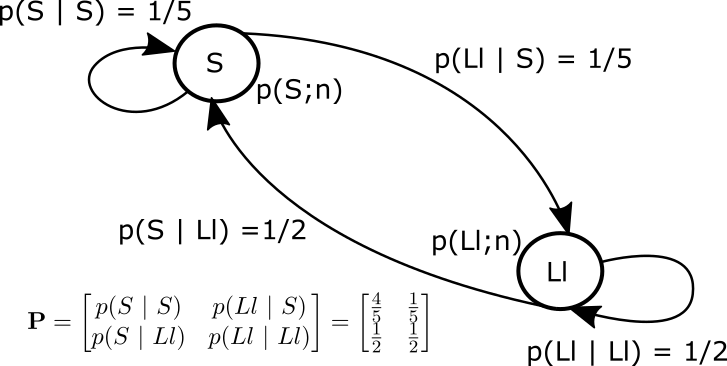
\includegraphics{diagramaEstados.png}
\caption{diagramaEstados.png}
\end{figure}

    Adviértase que:

\begin{itemize}
\tightlist
\item
  La cadena es homogénea. Por tanto, la matriz de transición (de un solo
  salto) se mantiene constante a lo largo del tiempo
\end{itemize}

\[
\mathbf{P} = 
\begin{bmatrix}
p(S\ |\ S) & p(Ll\ |\ S)\\
p(S\ |\ Ll) & p(Ll\ |\ Ll)
\end{bmatrix} = 
\begin{bmatrix}
\frac{4}{5} & \frac{1}{5}\\
\frac{1}{2} & \frac{1}{2}
\end{bmatrix}
\]

\begin{itemize}
\tightlist
\item
  La matriz para \(k\) saltos sería, por tanto,
  \(\mathbf{P}(k)=\mathbf{P}^k\)
\item
  Las probabilidades de los estados en cada instante \(n\) se recogen en
  el vector \(\boldsymbol{\pi}(n)=[P(S; n), P(Ll;n)]\)
\item
  La secuencia no tiene por qué ser estacionaria, esto es, las
  probabilidades de los estados van variando conforme sea la matriz de
  transición
\end{itemize}

\[
\boldsymbol{\pi}(n+1) = \boldsymbol{\pi}(n+1)\mathbf{P}
\]

    La probabilidad de que un día \(n\) sea soleado es
\(P(S; n) = \frac{2}{3}\). Por tanto, la probabilidad de que sea
lluvioso es \(P(Ll; n) = 1-P(S; n) = \frac{1}{3}\), esto es:

\[
\boldsymbol{\pi}(n) = [\frac{2}{3}, \frac{1}{3}]
\]

Y, por tanto, las probabilidades de los estados al día siguiente es

\[
\boldsymbol{\pi}(n+1) = [\frac{2}{3}, \frac{1}{3}] \begin{bmatrix}
\frac{4}{5} & \frac{1}{5}\\
\frac{1}{2} & \frac{1}{2}
\end{bmatrix} = 
[\frac{21}{30}, \frac{9}{30}]
\]

Y a los dos días:

\[
\boldsymbol{\pi}(n+2) = [\frac{2}{3}, \frac{1}{3}] \begin{bmatrix}
\frac{4}{5} & \frac{1}{5}\\
\frac{1}{2} & \frac{1}{2}
\end{bmatrix}^2 = 
[\frac{2}{3}, \frac{1}{3}]
\begin{bmatrix}
\frac{37}{50} & \frac{13}{50}\\
\frac{13}{20} & \frac{7}{20}
\end{bmatrix} 
\]

    En el apartado (2) del enunciado hay tres instantes de tiempo que
considerar: Ayer, Hoy, Mañana

\begin{itemize}
\tightlist
\item
  La matrices de transición de ayer a hoy y de hoy a mañana son la
  misma: \(\mathbf{P}\)
\item
  La matriz de transición de ayer a mañana es \(\mathbf{P}^2\)
\end{itemize}

Por tanto

\begin{itemize}
\tightlist
\item
  La probabilidad de que mañana haga sol si ayer también hizo sol es
  \(\frac{37}{50}\)
\item
  La probabilidad de que mañana haga sol si ayer llovió es
  \(\frac{13}{20}\)
\end{itemize}

En el apartado (3) simplemente nos preguntan las probabilidades totales
de sol y de lluvia de un día, dadas las probabilidades totales del día
anterior:

\begin{itemize}
\tightlist
\item
  La probabilidad total de que haga sol es
  \(\frac{21}{30}=\frac{7}{10}\)
\item
  La probabilidad total de que haga sol es \(\frac{9}{30}=\frac{3}{10}\)
\end{itemize}

    La distribución estacionaria
\(\boldsymbol{\pi_\infty}=[P(S;\infty), P(Ll;\infty)]\) debe cumplir:

\[
\boldsymbol{\pi_\infty} = \boldsymbol{\pi_\infty}\mathbf{P}
\]

Sujeto a que \([P(S;\infty), P(Ll;\infty)] = 1\):

Resolviendo la ecuación resulta que

\[
P(S;\infty) = \frac{5}{7}\\
P(Ll;\infty) = \frac{2}{7}  
\]

Y, por tanto, existe la distribución estacionaria
\(\boldsymbol{\pi_\infty}=[\frac{5}{7}, \frac{2}{7}]\)


    % Add a bibliography block to the postdoc
    
    
    
    \end{document}
